  \section{Podstawy teoretyczne}
  
  \subsection{Rezonans stochastyczny}
  
  Rezonans stochastyczny (SR) jest zjawiskiem występującym (między innymi, na potrzeby niniejszej pracy) w układach pobudzanych co najmniej dwoma sygnałami, z których jeden jest periodyczny, drugi natomiast jest szumem. O występowaniu rezonansu stochastycznego mówimy, kiedy nałożenie sygnału periodycznego i niezerowego szumu na wejściu układu skutkuje wysoką periodycznością sygnału wyjściowego.
  
  Powyższe oznacza, że odpowiednio dobrany szum potrafi wzmacniać i wydobywać z układu sygnał periodyczny. Szum, zazwyczaj traktowany jako zjawisko niepożądane ze względu na obniżanie dokładności pomiaru, w układach z rezonansem stochastycznym staje się zjawiskiem jak najbardziej pożądanym. 
  
  Podstawową wielkością używaną przy badaniu rezonansu stochastyznego jest stosunek sygnału do szumu (signal-to-noise ratio, zwany dalej SNR), określający skuteczność wzmocnienia składowej periodycznej w wyniku działania szumu.

  Istnieje wiele układów z rezonansem stochastycznym, od podwójnej studni potencjału, przez układy progowe po układy równań różniczkowych.

  \subsubsection{Układ bistabilny}
  \label{sec:uklad_bistabilny}

  Najprostszym w rozpatrywaniu analitycznym rezonatorem stochastycznym jest cząstka poruszająca się w  podwójnej studni potencjału, opisywanej równaniem \cite{mcnamara}

  \begin{equation} \label{sr:1}
    V_t(x) = \frac{b}{4} x^4 - \frac{a}{2} x^2 + \lambda_0 x cos(\beta t)
  \end{equation}

  gdzie t jest czasem (modulacja potencjału w czasie), a $\lambda_0 > 0$ amplitudą modulacji dobraną tak, że potencjał $V_t(x)$ ma zawsze dwa lokalne minima. Taki model nazywa się asymetrycznym potencjałem podwójnej studni i zmienia się on w sposób ciągły w czasie z okresem $T_0 = \frac{2 \pi}{\beta}$.

  Sygnał periodyczny moduluje względną wysokość obu studni poencjału, tak że przez pierwszą połowę okresu głębsza jest ''prawa'' ($x>0$), a przez drugą połowę okresu -- ''lewa'' ($x<0$) studnia potencjału.

  Jeśli zobrazować sygnał wejściowy jako podnoszący minima potencjału, to schematycznie można przedstawić taki układ następująco (rys. \ref{fig:graphics:double_well}).

  \begin{figure}
    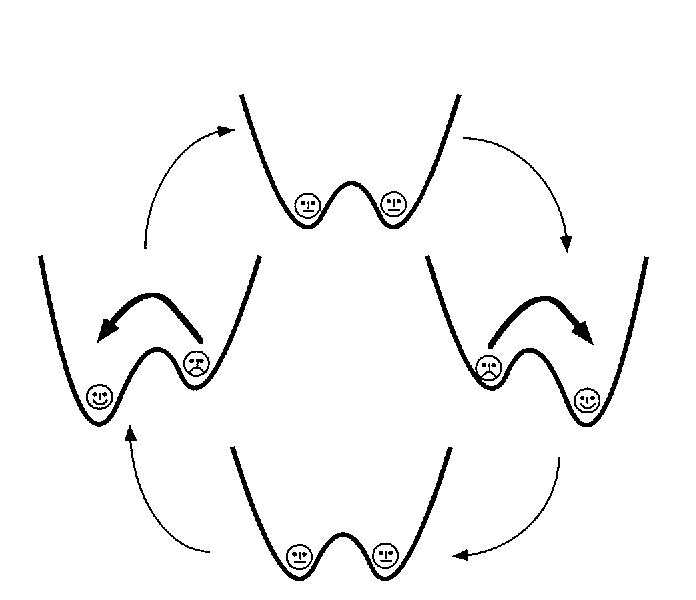
\includegraphics[width=80mm]{images/sr.jpg}
    \caption{obrazowe przedstawienie rezonansu stochastycznego w podwójnej studni potencjału}
    \label{fig:graphics:double_well}
  \end{figure}

  W przypadku silnego tłumienia równanie ruchu cząstki w modulowanym potencjale bistabilnym w obecności szumu ma postać

  \begin{equation} \label{sr:2}
    \dot x = - \partial_x V_t(x) + \xi (t)
  \end{equation}

  czyli przy danym w ~\ref{sr:1} potencjale ruch cząstki opisuje równanie Langevina

  \begin{equation} \label{sr:3}
    \dot x = -bx ^3 + ax + \lambda_0 cos(\beta t) + \xi (t)
  \end{equation}

  gdzie $\xi (t)$ jest białym (nieskorelowanym) szumem gaussowskim o natężeniu D

  \begin{equation} \label{sr:noise_correlation}
    \langle \xi(t) \xi(s) \rangle\ = 2 D \delta (t-s)
  \end{equation}

  Prawdopodobieństwo (na jednostkę czasu) że, przy braku sygnału periodycznego, cząstka znajdująca się w jednej ze studni potencjału przeskoczy do drugiej pod wpływem szumu dane jest wzorem Kramersa (tzw. Kramers rate)

  \begin{equation} \label{sr:kramers_rate}
    t^{-1}_K (D) = r_K (D) = 2 \pi \sqrt{|V''(x_{min})| |V''(x_{max})|} e^{-\frac{\Delta V}{2D}}
  \end{equation}

  gdzie $x_{min}$ i $x_{max}$ oznaczają położenia odpowiednio lokalnego minimum i maksimum potencjału, a $\Delta V = V(x_{max}) - V(x_{min})$ jest wysokością bariery potencjału.

  Dodanie sygnału periodycznego moduluje prawdopodobieństwo \ref{sr:kramers_rate} tak, że przez pierwszą połowę okresu większe jest prawdopodobieństwo przeskoku ze studni lewej (w tej połowie okresu płytszej) do prawej (w tej połowie okresu głębszej), a przez drugą połowę - odwrotnie.

  Jako sygnał wyjściowy przyjmuje się sygnał o wartościach dyskretnych odzwierciedlających w której ze studni potencjału przebywa cząstka:

    \begin{equation}
    y(t) = 
    \begin{cases}
      -1 & \text{dla } x(t) < 0 \\
      -1 & \text{dla } x(t) > 0 
    \end{cases}
  \end{equation}

  Niech $\langle y(t) \rangle$ oznacza sygnał $y(t)$ uśredniony po wielu okresach sygnału periodycznego. Widmo mocy takiego sygnału

  \begin{equation} \label{sr:power_spectrum}
    S(\beta) = |Y(\beta)|^2 = |\int_{-T}^T \langle y(t) \rangle e^{-i \beta t} dt |^2
  \end{equation}

  składa się z szerokiego tła szumowego oraz pików dla częstości $\beta$ %i jej nieparzystych wielokrotności%
  , co obrazuje rys. \ref{fig:graphics:mcnamara8}.

  \begin{figure}
    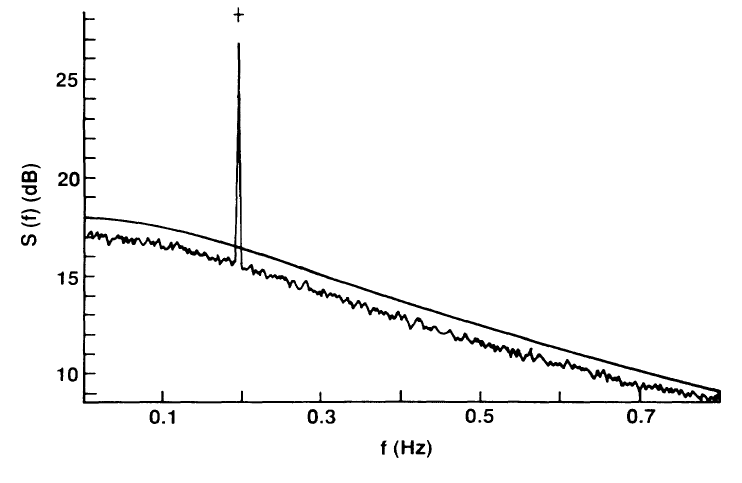
\includegraphics[width=100mm]{images/mcnamara_8.png}
    \caption{Widmo mocy $S(f)$ cząstki w podwójnej studni potencjału. Częstotliwość modulacji $f_s = \frac{\beta}{2 \pi} = 0.195$, $a=32$, $\Delta V = 256$, $\lambda_0 = 8$, $D = 256$ i $\Delta t = 0.005$. Sygnał teoretyczny (krzyżyk) i wyniki symulacji różnią się o około 1dB. (za: McNamara, Wiesenfeld \cite{mcnamara})}
    \label{fig:graphics:mcnamara8}
  \end{figure}

  Stosunek sygnału do szumu

  \begin{equation} \label{sr:snr}
    SNR = 10 log \frac{S(\beta)}{S_N(\beta)}
  \end{equation}

  (gdzie $S_N(\beta)$ oznacza wartość tła szumowego w widmie mocy w okolicach wartości sygnału periodycznego) ma maksimum jako funkcja nateżęnia szumu SNR(D). Patrz też rys. \ref{fig:graphics:mcnamara9b}

  \begin{figure}
    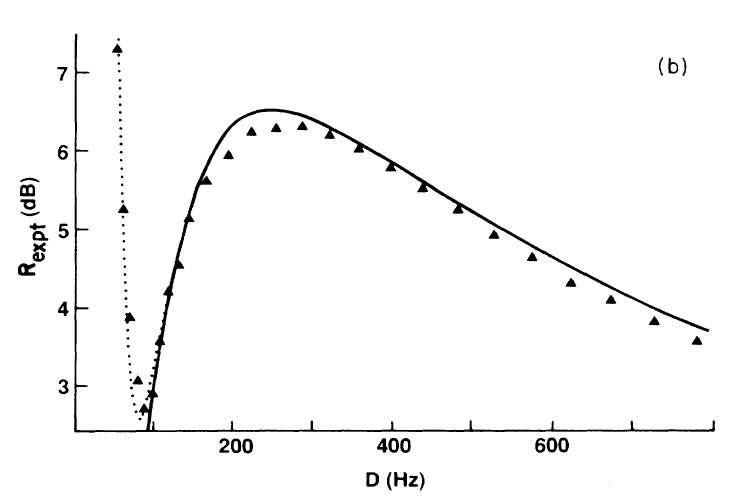
\includegraphics[width=100mm]{images/mcnamara_9b.png}
    \caption{SNR (oznaczony tutaj jako $R_{expt}$) jako funkcja wariancji szumu D. Parametry takie jak użyte do rys. \ref{fig:graphics:mcnamara8} (za: McNamara, Wiesenfeld \cite{mcnamara})}
    \label{fig:graphics:mcnamara9b}
  \end{figure}

  Maksimum SNR odpowiada w przybliżeniu takiemu natężeniu szumu, że dwa ''przejścia'' pomiędzy studniami przypadają na jeden okres modulacji periodycznej. Odpowiada to zrównaniu się czasu Kramersa (średni czas przebywania w jednej studni; odwrotność współczynnika Kramersa $r_K$) z połową okresu sygnału periodycznego \cite{fauve}:

  \begin{equation} \label{sr:kramers}
    t_K = r_{K}^{-1} \approx \frac{T_0}{2}
  \end{equation}  

  Dokładniejsze obliczenia w przybliżeniu adiabatycznym (założenie częstości sygnału periodycznego o wiele mniejszej od czasu relaksacji układu $\beta \ll \tau^{-1}_r$) pozwalają uzyskać dokładniejszy wzór na SNR (za \cite{mcnamara}):

  \begin{equation} \label{sr:snr_theoretical}
    SNR(D) = \frac{\sqrt{2}a \lambda^{2}_0 c^2}{D^2} e^{-\frac{\Delta V}{2D}}
  \end{equation}

  Wzór ten dobrze opisuje wyniki symulacji numerycznych, przedstawionych na rys. \ref{fig:graphics:mcnamara9b}.



  \subsubsection{Układ progowy}
  \label{sec:uklad_progowy}

  W zastosowaniach praktycznych (wzmacnianie sygnałów) oraz symulacjach popularny jest rezonator monostabilny, progowy (układ niedynamiczny). Mechanizm jego działania polega na wysłaniu przez układ ''szpilki'' potencjału kiedy suma sygnału periodycznego i szumu przekroczy (wznosząco) wartość progową. Taki rezonator był badany doświadczalnie (symulacje, realizacja elektroniczna) i teoretycznie w pracy \cite{gingl_kiss_moss}. Widmo mocy takiego układu posiada wysokie i wąskie piki dla częstotliwości wejściowego sygnału i jej wszystkich (parzystych i nieparzystych) wielokrotności.

  Sygnał wejściowy w układzie badanym przez Gingla \cite{gingl_kiss_moss} jest po prostu sumą sygnału periodycznego i szumu:

  \begin{equation} \label{sr:gingl}
    v_{in}(t) = A sin (\omega_0 t) + D \xi(t)
  \end{equation}
  
  Wyniki uzyskane przez Gingla \emph{et al.} przedstawia rys. \ref{fig:graphics:gingl}. 

  \begin{figure}
    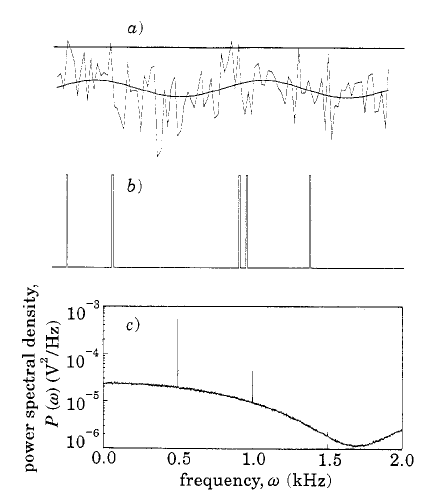
\includegraphics[width=100mm]{images/gingl_1.png}
    \caption{Numeryczna reprezentacja niedynamicznego rezonansu stochastycznego. a) Sygnał koherentny, sygnał periodyczny i szum gaussowski, poniżej progu zaznaczonego linią. Odległość pomiędzy linią progu a średnią sygnału periodycznego jest równa wysokości progu. b) Przebieg czasowy impulsów odpowiadających przekraczaniu (''w górę'') progu przez sumę sygnałów. c) Znormalizowane widmo mocy przebiegu impulsów (za: Gingl, Kiss, Moss \cite{gingl_kiss_moss} )}
    \label{fig:graphics:gingl}
  \end{figure}

  \begin{figure}
    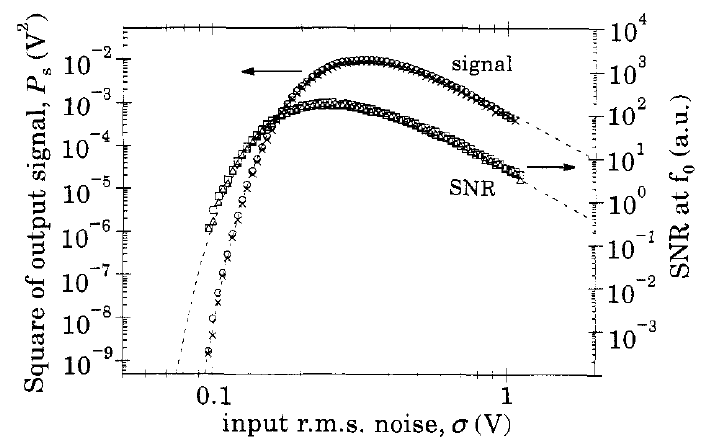
\includegraphics[width=120mm]{images/gingl_2.png}
    \caption{Wyniki eksperymentów z szumem białym przeprowadzonych przez Gingla \emph{et al.} (punkty) oraz krzywe obliczone teoretycznie (linie przerywane) na układzie progowym. Sygnał wejściowy: $\lambda_0 = 0.1V$, $f_0 = 38 Hz \text{i } 305 Hz $, szum biały, $U_t = 0.45V$. $\triangle$ i $\times$ 305 Hz, $\circ$ i $\Box$ 38Hz. Linie przerywane: krzywe dopasowane według \ref{sr:gingl:snr}. (za: Gingl, Kiss, Moss \cite{gingl_kiss_moss} )}
    \label{fig:graphics:gingl2}
  \end{figure}

  Przed przystąpieniem do eksperymentów Gingl \emph{et al.} wyprowadzili teoretyczny wzór na SNR układu przy spełnieniu pewnych założeń (przybliżenie adiabatyczne, sygnał periodyczny wolnozmienny i słabszy niż średnia kwadratowa szumu), korzystając z twierdzenia Campbella i wzoru Rice'a (na przejścia przez zero) \cite{rice}

  \begin{equation} \label{sr:gingl:snr}
    SNR = \nu_0 (\lambda_0 U_t)^2 \sigma ^{-4} exp [-(U_t/{\sigma})^2 / 2]
  \end{equation}

  W powyższym wzorze $\lambda_0$ jest amplitudą sygnału periodycznego, $\nu_0$ średnią częstotliwością jednokierunkowych przejść przez zero (obliczoną z wzoru Rice'a), a $\sigma$ jest średnią kwadratową szumu.

  Pomimo różnic w badanym układzie, kształt krzywej $SNR(\sigma)$ oraz wyniki eksperymentów przeprowadzonych przez Gingla \emph{et al.} odpowiadają kształtowi tej krzywej dla układu w studni bistabilnej, patrz rys. \ref{fig:graphics:gingl2}.


  Rezonator badany przez Gingla \emph{et al.} generuje na wyjściu wąski pik o stałej szerokości kiedy sygnał zaszumiony gwałtownie wzrasta przekraczając próg (''rising peak'').

  Nieco inny rezonator progowy badany był w pracach \cite{blondeau_e53} i \cite{blondeau_e55}. Układ ten produkuje pik o szerokości równej czasowi trwania impulsu (a dokładniej: czasowi, przez jaki wartość sygnału przekracza wartość progową). Sygnał wyjściowy z takiego rezonatora ma postać ma postać:

  \begin{equation} \label{sr:gingl2}
    v_{out}(t) = \Gamma[A sin (\omega_0 t) + D \xi(t) - \theta]
  \end{equation}

  gdzie $\theta$ jest progiem, a $\Gamma(u)$ jest funkcją Heaviside'a ($\Gamma(u) = 0$ dla $u \leq 0$, $\Gamma(u) = 1$ dla $u > 0$).

  Oba sposoby uzyskiwania sygnału wyjściowego skutkują bardzo zbliżonym widmem mocy i wprowadzają podobne (choć wynikające z innej cechy zastosowanej metody) niewielkie rozmycie piku głównego w widmie mocy.

  Warto wspomnieć, że układ opisany w pracy Chapeau, Blondeau \cite{blondeau_e53}, czyli układ progowy z nieliniowością typu Heaviside'a, można traktować jako model neuronu klasycznego (binarnego) z sygnałem periodycznym i szumem.

  \subsubsection{Wzmocnienie SR przez sprzężenie}
  \label{sec:wzmocnienie_przez_sprzezenie}

  Bardzo dobrą strategią wzmocnienia SR -- czyli zwiększenia signal-to-noise ratio -- jest zbudowanie układu kilku identycznych rezonatorów, połączonych ze sobą i wymieniających sygnał. Rezonans stochastyczny w takim układzie nazywany jest ''Array Enhanced Stochastic Resonance'' (AESR) \cite{lindner_meadows} i, przy optymalnym doborze parametrów układu, jest silniejszy (w sensie wyższej maksymalnej wartości SNR w funkcji natężenia szumu) niż SR w pojedynczym rezonatorze.

  Dotychczas badano AESR głównie w układach przestrzennie rozciągłych. Zbadano m.in. obowiązujące w takich układach reguły skalowania \cite{lindner_meadows} \cite{tanabe_shimokawa}, wpływ przesunięcia fazowego wymuszenia periodycznego w poszczególnych rezonatorach (związanego z rozciągłością przestrzenną układu) \cite{ijmpb_14_8} oraz kompensację ww. przesunięcia opóźnieniem w transmisji sygnału pomiędzy rezonatorami \cite{ijmpb_23_2}. W większości dotychczasowych prac badano proste rezonatory, takie jak neurony dyskretne i inne układy progowe. Pewnym wyjątkiem jest tu praca \cite{tanabe_shimokawa}, której autorzy badali duże (tysiące rezonatorów) macierze aktywnych rotatorów \cite{wiesenfeld} \cite{pakdaman}.

  Wyniki uzyskane w badanych dotychczas układach (i przedstawione w cytowanych wyżej pracach) wykazywały, że zbudowanie macierzy oddziałujących rezonatorów istotnie wpływa na maksymalizację SNR przy odpowiednim doborze parametrów układu.

  W pracy \cite{lindner_meadows} zbadano jednowymiarowy układ (łańcuch) sprzężonych dyfuzyjnie bistabilnych rezonatorów stochastycznych, pobudzanych wspólnym sygnałem periodycznym i nieskorelowanymi przestrzennie szumami stochastycznymi

  \begin{equation}
    \dot x_i = -x_i^3 + x + \lambda_0 cos(\beta t) + k(x_{i+1} + x_{i-1} -2 x_{i}) + \xi_i (t)
  \end{equation}

  gdzie $\xi(t)$ to szum nieskorelowany, jak w \ref{sr:noise_correlation}, $i$ jest indeksem rezonatorów w łańcuchu ($ i = 1,2,3...N$), a $k$ oznacza stałą sprzężenia (przyjęto periodyczne warunki brzegowe).

  Wykazano, że optymalne natężenie szumu, przy którym obserwuje się maksimum SNR w pojedynczym rezonatorze, zależy od k i długości łańcucha N. Maksimum SNR w funkcji szumu w zasadzie rośnie z długością łańcucha N przy ustalonym sprzężeniu k. Natomiast przy ustalonej długości łańcucha N istnieje optymalna wartość sprzężenia k, dla której maksimum SNR w funkcji szumu przyjmuje najwyższą możliwą wartość.

  Zjawisko AESR związane jest z synchronizacją czasowo-przestrzenną przeskoków pomiędzy studniami potencjału we wszystkich rezonatorach, do której [synchronizacji] dochodzi przy optymalnym sprzężeniu i wartości szumu, odpowiadającej maksimum SNR.

  Interesującym zjawiskiem jest coraz mniejszy przyrost maksimum SNR w miarę rozbudowywania układu o kolejne rezonatory: nie jest to wzrost asymptotyczny do pewnej wartości progowej, a po prostu spowolnienie jego przyrostu (wykresy uzyskane w pracy \cite{lindner_meadows} wykazują podobieństwo do zależności logarytmicznej). Wynika z tego, że optymalny przyrost SNR jest do osiągnięcia już w macierzy kilku bądź kilkunastu rezonatorów. Wyniki Lindnera et. al. \cite{lindner_meadows} przedstawia rysunek ~\ref{fig:graphics:lindner_meadows}.

  \begin{figure}
    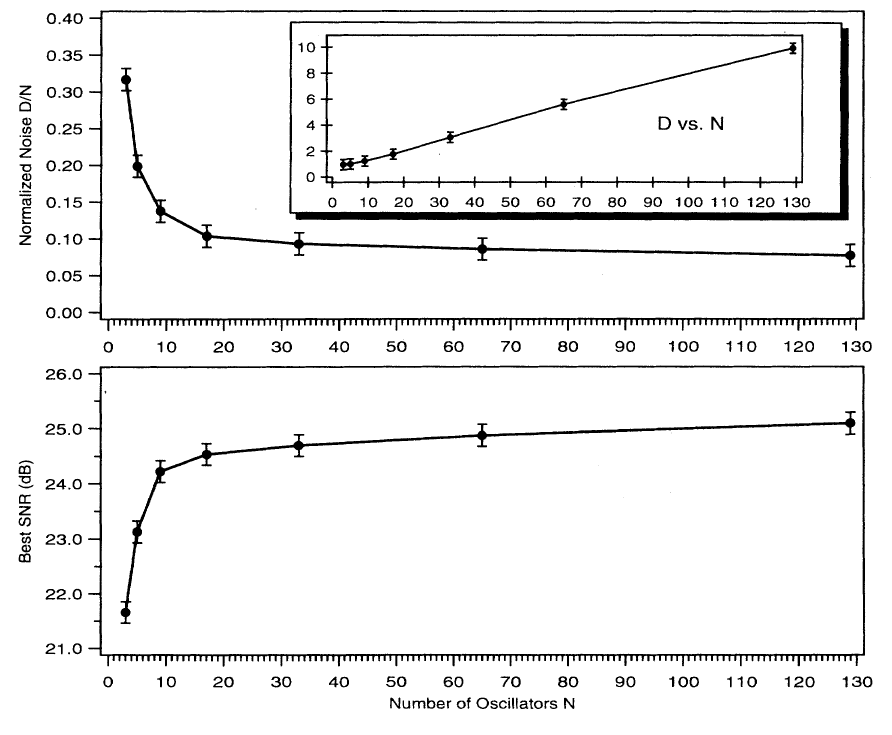
\includegraphics[width=120mm]{images/lindner_meadows.png}
    \caption{Fig. 4 z pracy Lindnera et al. \cite{lindner_meadows}. Relacje skalowania znormalizowanego szumu oraz SNR w miarę przyrostu liczby połączonych w macierz rezonatorów. (a) wartość szumu (znormalizowana do N) dla której występuje maksimum SNR, (b) wartość maksimum SNR przy optymalnie dobranym sprzężeniu k}
    \label{fig:graphics:lindner_meadows}
  \end{figure}

  Budowanie macierzy połączonych rezonatorów, jako posunięcie zorientowane na maksymalizację SNR, można uznać za jedną z metod kontroli SR.

  Ponieważ sygnały periodyczne (np. fale biegnące) rozchodzą się ze skończoną prędkością, w układach przestrzennie rozciągłych sygnały docierające do poszczególnych rezonatorów mogą być przesunięte w fazie. Więcej informacji na temat SR w takich układach zawiera rozdział ~\ref{sec:przesuniecie_fazy}.

  \subsubsection{Kontrola SR}
  
  Podobnie jak w przypadku innych układów nieliniowych badane były możliwości kontroli rezonansu stochastycznego (czyli technik maksymalizacji SR). 

  W pracy Gammaitoniego i in. \cite{gammaitoni} badano układ progowy (zbudowany na przerzutniku Schmitta) i kontrolowano SR poprzez modulację progu, czyli jest to metoda kontroli bez sprzężenia zwrotnego. 

  Przerzutnik Schmitta jest układem elektronicznym działającym analogicznie do bistabilnej studni potencjału. Wyjście układu przyjmuje jedną z dwóch wartości (odpowiednik stanów) w zależności od przekroczenia (bądź nie) pewnego progu przez napięcie wejściowe, co odpowiada układowi opisanemu w rozdziale \ref{sec:uklad_bistabilny}. Modulowanie progu zadziałania jest odpowiednikiem modulowania wysokości bariery potencjału pomiędzy studniami w układzie bistabilnym.

  %\begin{figure}
  %  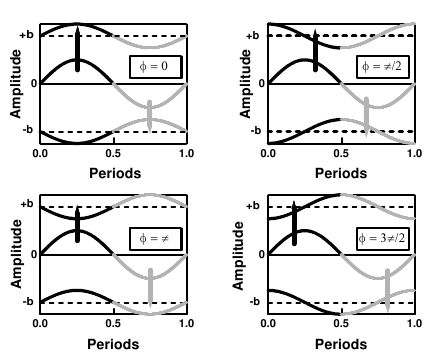
\includegraphics[width=100mm]{images/gammaitoni_1.png}
  %  \caption{Sygnał wejściowy S(t) (środkowa krzywa) względem górnych i dolnych progów modulowanych dla czterech różnych przesunięć fazowych. Częstotliwości sygnału i modulacji progów są sobie równe $\omega_M = \omega_S$. Kolory czarny i szary oddzielają połówki cyklu działania. Strzałki wskazują najbardziej prawdopodobny moment przełączenia. Za \cite{gammaitoni}}
  %  \label{fig:graphics:gammaitoni:fig1}
  %\end{figure}

  \begin{figure}
    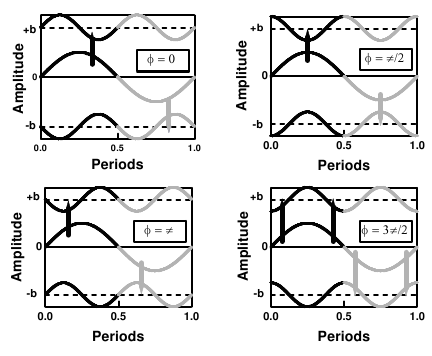
\includegraphics[width=100mm]{images/gammaitoni_2.png}
    \caption{Sygnał wejściowy S(t) (środkowa krzywa) względem górnych i dolnych progów modulowanych dla czterech różnych przesunięć fazowych. Częstotliwość modulacji progów $\omega_M$ jest dwa razy większa od częstotliwości sygnału $\omega_S$, tj. $\omega_M = 2 \omega_S$. Kolory czarny i szary oddzielają połówki cyklu działania. Strzałki wskazują najbardziej prawdopodobny moment przełączenia. Za \cite{gammaitoni}}
    \label{fig:graphics:gammaitoni:fig2}
  \end{figure}

  W pracy \cite{gammaitoni} największe wzmocnienie wyjściowego osiągnięto SNR dla częstotliwości modulacji progu równej dwukrotności częstotliwości sygnału $\omega_M = 2 \omega_S$ i różnicy faz równej $\pi/2$ -- patrz rys. \ref{fig:graphics:gammaitoni:fig2}.

  W niniejszej pracy badam inną metodę kontroli rezonansu stochastycznego, poprzez maksymalizację periodyczności sygnału odbieranego od sąsiadujących w sieci neuronów.
  
  \subsection{Modele neuronów biologicznych}
  
  Pobudzenie układu nerwowego zwierzęcia wywołuje zmienne w czasie prądy jonowe w membranach neuronów czuciowych, które w konsekwencji wywołują potencjały czynnościowe (''szpilki'' potencjału elektrycznego) w momencie depolaryzacji membrany.
  
  Modele neuronów czuciowych (sensory neuron model, SNM), podobnie jak neuronów binarnych używanych w badaniu sieci neuronowych, wykazują bistabilność, tzn. istnienie dwóch stanów stabilnych, w których układ może przebywać. Podstawową różnicą jest ciągły potencjał (napięcie) SNM, co oznacza traktowanie stanów stabilnych jako zakresów (zamiast pojedynczych wartości), pomiędzy którymi układ przechodzi poprzez stany niestabilne. 
  
  Naturalną konsekwencją ciągłego potencjału jest użycie równań różniczkowych (zamiast różnicowych, jak w neuronach binarnych) w matematycznym opisie SNM. Oprócz potencjału w wielu SNM istnieje równanie różniczkowe na drugą zmienną układu, ujemnie wpływającą na pochodną potencjału, zwaną dalej relaksacją.
  
  Pierwszym nowoczesnym SNM który dobrze opisywał powstawanie i propagację potencjałów czynnościowych w układzie biologicznym (olbrzymim aksonie kałamarnicy) jest model Hodgkina-Huxleya \cite{hodgkin}, za który w roku 1963 twórcy zostali uhonorowani nagrodą Nobla. Jest to model skomplikowany, o dużej liczbie zmiennych, postulujący traktowanie membrany komórkowej jako obwodu elektrycznego.

  \begin{figure}
    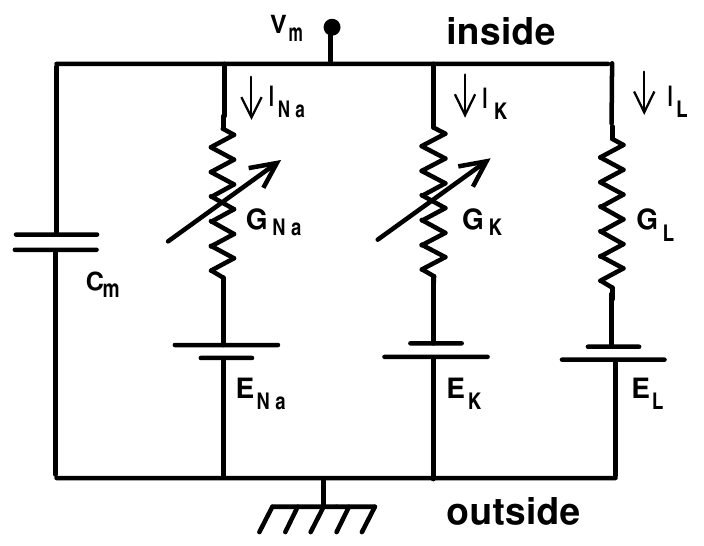
\includegraphics[width=100mm]{images/hh.png}
    \caption{Przedstawienie modelu Hodgkina-Huxleya, za ''Book of GENESIS'' \cite{genesis}}
    \label{fig:graphics:genesis}
  \end{figure}

  Posługując się oznaczeniami z rysunku \ref{fig:graphics:genesis}, w modelu Hodgkina-Huxleya $C_{m}$ pełni rolę pojemności membrany lipidowej, natomiast na łączny prąd jonowy $I_{ion}$ składają się trzy prądy: sodowy $I_{Na}$, potasowy $I_{K}$ i upływu $I_{L}$ (realizowany głównie przez jony chlorkowe).

  W postaci ogólnej równanie różniczkowe opisujące taki obwód przedstawia się następująco

  \begin{equation} \label{hh:1}
    C_{m} \frac{dV_{m}}{dt} + I_{ion} = I_{ext}
  \end{equation}

  gdzie $C_{m}$ to wspomniana już wyżej pojemność membrany, $V_{m}$ to potencjał wewnątrzkomórkowy (potencjał membrany), $I_{ion}$ to łączny prąd jonowy, a $I_{ext}$ jest przyłożonym z zewnątrz prądem.

  Konwencja przyjęta w modelu H-H oznacza, że prąd jonowy i zewnętrzny mają przeciwne znaki. Przekłada się to na następujące zachowanie: dodatni prąd $I_{ext}$ będzie depolaryzował komórkę (zwiększał $V_{m}$), podczas kiedy dodatni prąd $I_{ion}$ będzie powodował nadpolaryzowację neuronu (zmniejszał $V_{m}$). Zgodnie z tą konwencją wpływ dodatnich jonów jest traktowany jako prąd ujemny, czyli odwrotnie niż klasyczne rozumienie prądu w teorii obwodów (dodatni prąd jest przepływem dodatnich ładunków). Taka konwencja dla prądów jonowych nosi nazwę \emph{konwencji fizjologów} i wynika z tego, że badanie prądów jonowych nie polega na mierzeniu prądu jonowego wewnątrz komórki (co jest eksperymentalnie bardzo trudne), tylko na pomiarze prądu przyłożonego (zewnętrznego) potrzebnego do zneutralizowania prądu jonowego.

  W oryginalnej pracy Hodgkin i Huxley depolaryzacja oznaczała spadek napięcia membrany. Współczesna konwencja, przyjęta także w niniejszej pracy, jest odwrotna: depolaryzacja zwiększa napięcie membrany $V_{m}$.

  Choć opisywany względnie prostymi równaniami, model Hodgkina-Huxleya jest dla zastosowań symulacyjnych złożony i niezbyt praktyczny (konieczność modelowania i śledzenia każdego z prądów jonowych wraz z dobieraniem zespolonej rezystancji każdego z kanałów). Wśród modeli uproszczonych najpopularniejszy jest model neuronu FitzHugh-Nagumo.


  \subsubsection{Model Neuronu FitzHugh-Nagumo}

  Model FitzHugh-Nagumo (FHN) \cite{fitzhugh}, będący podstawą niniejszej pracy, modeluje potencjał neuronu jako układ dwóch równań różniczkowych z jedną zmienną losową:

  \begin{equation}
    \epsilon \frac{dv}{dt} = v - v^3 - \omega + I_{ext}
  \end{equation}

  \begin{equation}
    \frac{d \omega}{dt} = v - d \omega - b
  \end{equation}

  W modelu FHN $v(t)$ pełni rolę szybkozmiennego ''potencjału'' (odpowiednik biologicznego potencjału czynnościowego neuronu), natomiast $\omega (t)$ pełni rolę wolnozmiennej ''relaksacji''. $I_{ext}$ to pobudzenie zewnętrzne. $\epsilon$ to większe od zera i mniejsze od jedności skalowanie czasu, które sprawia że $v(t)$ jest szybszą zmienną w tym układzie.


  Model użyty w niniejszej pracy ma zmodyfikowaną postać, zaproponowaną przez A. Longtina \cite{longtin}. Zewnętrzne pobudzenie jest w tej wersji rozbite na szum $\xi(t)$ oraz sygnał periodyczny $r sin(\beta t)$.

  \begin{equation} \label{eq:v}
    \epsilon \frac{dv}{dt} = v(v-a)(1-v)- \omega + \xi(t)
  \end{equation}

  \begin{equation} \label{eq:w}
    \frac{d \omega}{dt} = v - d \cdot \omega - [b + r sin(\beta t)]
  \end{equation}

  Szum używany pierwotnie w systemach bistabilnych $\xi(t)$ jest białym szumem gaussowskim o zerowej średniej, nieskorelowanym $\langle \xi(t) \xi(s) \rangle\ = 2 D \delta (t-s)$ (patrz też rozdział \ref{sec:uklad_bistabilny}). W pracy Longtina, dla możliwości sterowania czasem korelacji szumu $\tau_c = \lambda^{-1}$, został on zastąpiony przez $\eta(t)$, szum skorelowany generowany w procesie Ornsteina-Uhlenbecka:

  \begin{equation} \label{eq:eta}
    \frac{d \eta}{dt} = -\lambda \eta(t) + \lambda \xi(t)
  \end{equation}

  $d \cdot \omega$ po prawej stronie równania \ref{eq:w} jest pomnożeniem $\omega$ przez parametr $d$, a nie różniczką. 

  %(REFERAT O ZAKRESIE STOSOWALNOŚCI PARAMETRÓW?)
  

  \subsubsection{Przekształcenia modelu FHN}

  Równania \ref{eq:v}, \ref{eq:w} zawierają sygnał periodyczny zawarty w dynamice relaksacji, natomiast szum (element stochastyczny) w dynamice potencjału. Oryginalnym powodem takiego rozmieszczenia składowych sygnału zewnętrznego była łatwość porównania modelu stochastycznego z modelem deterministycznym (bez szumu) badanym w pracy Alexander \emph{et al.} \cite{alexander}. W pracy tej ściśle wykazano \cite{longtin}, że układ równań (\ref{eq:v}, \ref{eq:w}) jest równoważny układowi w postaci:

  \begin{equation}
    \epsilon \frac{dv}{dt} = v(v-a)(1-v)- \omega + A sin(\beta t) + \xi(t)
  \end{equation}

  \begin{equation}
    \frac{d \omega}{dt} = v - d \omega - b
  \end{equation}

  tak długo, jak długo spełniona jest nierówność $\beta < \frac{1}{\epsilon}$.

  \subsubsection{Zachowanie progowe i wzmacnianie szumu w modelu FHN}

  Jedną z najważniejszych cech modelu FitzHugh-Nagumo jest jego progowe zachowanie, tzn. gwałtowny wzrost potencjału czynnościowego jeśli przekroczy on pewną wartość graniczną. W połączeniu z szumem oraz (słabym) sygnałem periodycznym model FHN pozwala zaobserwować rezonans stochastyczny, z wyraźnymi pikami w widmie mocy dla częstotliwości wymuszenia periodycznego i jej wielokrotności.

  %(WIĘCEJ CYTOWAŃ)

  W pracy \cite{longtin} Longtin dobrał zakres parametrów powyższych równań oraz otrzymał bardzo obiecujące wyniki. Znaleziony przezeń histogram interwałów czasowych pomiędzy ''szpilkami'' potencjału wyjściowego (Inter-Spike Interval Histogram, ISIH) był podobny do danych zebranych empirycznie podczas badania włókien nerwów słuchowych kota (rys. \ref{fig:graphics:longtin1b}, \ref{fig:graphics:longtin5a}).

  \begin{figure}
    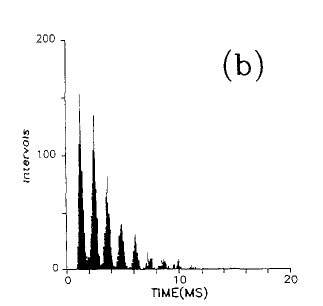
\includegraphics[width=80mm]{images/longtin_fig1b.png}
    \caption{ISIH we włóknach nerwów słuchowych kota, pobudzanych sygnałem o częstotliwości 800Hz i natężeniu 60dB. Za \cite{longtin}.}
    \label{fig:graphics:longtin1b}
  \end{figure}

  Dla optymalnego natężenia szumu D, odpowiadającego występowaniu R, w histogramie interwałów międzyszpilkowych pojawiają się ostre maksima, dla wartości odpowiadających okresowi pobudzenia periodycznego lub jego wielokrotnościom. Oznacza to, że pojawienie się ''szpilek'' potencjału czynnościowego jest zsynchronizowane z pobudzeniem periodycznym. Dla innych natężeń szumu maksima histogramu są niższe i rozmyte, co odpowiada miejszej synchronizacji pomiędzy aktywnością neuronu a pobudzeniem periodycznym.

  %Wyniki symulacji modelu FHN w pracy Longtina, z dokładnością do parametrów (częstotliwość sygnału periodycznego), okazały się bardzo zbliżone do danych empirycznych zebranych podczas badania organizmów żywych (por. wykresy).

  \begin{figure}
    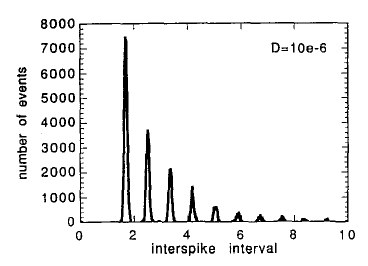
\includegraphics[width=80mm]{images/longtin_fig5a.png}
    \caption{ISIH w symulacji układu FHN. Okres sygnału periodycznego wynosi 0.84s ($\beta = 7.5$)}
    \label{fig:graphics:longtin5a}
  \end{figure}  


  %\subsubsection{ew. FHN-wariant bez szumu i bez period., goły}

  %Zachowanie modelu FHN w wariancie deterministycznym, tj. bez szumu, było przedmiotem pracy \cite{alexander}

  %(ZREFEROWAĆ? WYRZUCIĆ PODROZDZIAŁ?)

  \subsubsection{Rezonans Stochastyczny w macierzach rezonatorów ciągłych}

  Podobnie jak proste rezonatory (patrz rozdział \ref{sec:wzmocnienie_przez_sprzezenie}), także rezonatory ciągłe (w tym neurony FitzHugh-Nagumo) łączono w macierz, celem zbadania dynamiki takiego układu i maksymalizacji periodyczności sygnału wyjściowego. 

  Badania macierzy ciągłych rezonatorów zostały przeprowadzone przez Tanabe \emph{et al.} i opisane w pracy \cite{tanabe_shimokawa}. Badane były duże (kilka tysięcy elementów) macierze aktywnych rotatorów (AR), jako prostszych w analizie teoretycznej i zarazem posiadających podobną dynamikę jak modele neuronów FitzHugh-Nagumo i Hodgkin-Huxley. Równanie opisujące dynamikę AR zostało zaczerpnięte z pracy \cite{shinomoto} i rozszerzone o wpływ rotatorów połączonych w postaci pola średniego:

  \begin{equation}
    \frac{d \phi_i}{dt} = 1 - a sin(\phi_i) + \frac{G}{N} \sum\limits_{j=1}^{N} sin(\phi_j - \phi_i) + A sin(\Omega t) + \sigma \xi_i
  \end{equation}

  Gdzie $i=1,2,...N$, $\phi_i$ jest fazą rotatora, $a > 1$, $G \ge 0$ jest siłą połączenia, $\sigma$ jest natężeniem szumu gaussowskiego $\xi_i$. Podobnie jak we wszystkich pracach zorientowanych na badanie SR, rozważano wyłącznie podprogowe poziomy wymuszenia periodycznego $sin(\Omega t)$.

  Symulacje rozpoczęto od bardzo małych wartości $\sigma$, najmniejszych wystarczających do zaobserwowania ''szpilek''. Wyniki obrazuje rysunek \ref{fig:graphics:tanabe}. Sygnałem wyjściowym z całego układu (macierzy rezonatorów) był współczynnik reakcji, zdefiniowany jako ułamek elementów przekraczających wartość $3 \pi / 2$ w krótkim zakresie. Dla małego poziomu szumu, jeśli następował ''strzał'' (gwałtowny wzrost fazy rotatora), to następował on w całej sieci jednocześnie - był synchroniczny w całej sieci, natomiast interwały pomiędzy strzałami były nieregularne. Zwiększanie poziomu szumu co prawda zwiększało regularność ''strzałów'' (regularne interwały), ale za to redukowało ich synchroniczność, co na rysunku \ref{fig:graphics:tanabe} objawia się rozmyciem ''szpilek'' współczynnika reakcji.

  Konkluzją pracy było poszukanie źródeł tak złożonych odpowiedzi w dynamice pojedynczego rezonatora. Istotnie, na poziomie nawet pojedynczego rezonatora, można wyodrębnić trzy zakresy dynamiki. Dla niskich poziomów szumu rezonator ''strzela'' sporadycznie i nieregularnie, natomiast jego strzały bardzo zależą od czynników zewnętrznych - np. maksimum sygnału periodycznego. Dla wysokich poziomów szumu ''strzały'' rezonatora są częste i nieregularne, mało zależne od czynników zewnętrznych, aż do przypadku skrajnego: rezonatora bez pobudzenia periodycznego, ''strzelającego'' pod wpływem samego szumu. Pomiędzy tymi dwoma zakresami istnieje trzeci, zakres umiarkowanego szumu, w którym ''strzały'' są regularne i dość częste, i w którym rezonator można traktować jako \emph{wewnętrzne} oscylatory perturbowane szumem. Zbadana przez Tanabe \emph{et al.} dynamika dużych macierzy rezonatorów odzwierciedla te zakresy i charakterystyczne w nich zachowania.

  \begin{figure}
    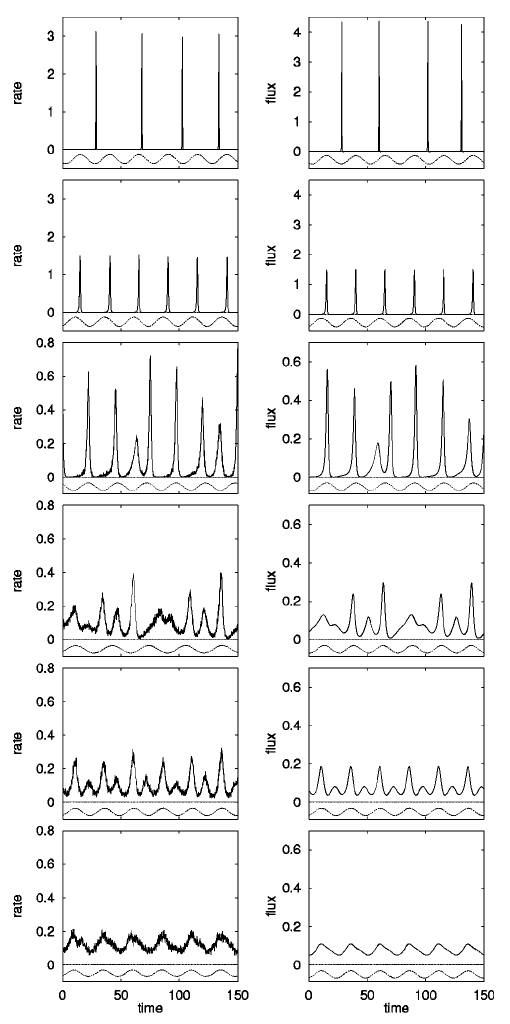
\includegraphics[width=80mm]{images/tanabe.png}
    \caption{Lewa kolumna: globalna aktywność macierzy AR złożonych z 10 000 rotatorów. Oś rzędnych przedstawia czas (ms), oś odciętych współczynnik ($ms^{-1}$) zdefiniowany jako ułamek elementów przekraczających wartość $3 \pi / 2$ w zakresie 0.1ms. Prawa kolumna: przepływ rozwiązania równiania Fokkera-Plancka przez wartość $3 \pi / 2$. Poziom szumu $\sigma$ rośnie ''z góry na dół''. Za \cite{tanabe_shimokawa}}
    \label{fig:graphics:tanabe}
  \end{figure}

  \subsection{Pamięć i Opóźnienie}
  
  Dotychczasowe badania (symulacje) układów neuronów FHN, choć dotyczyły układów neuronów połączonych (wymieniających sygnały, a dokładnie potencjał czynnościowy), nie brały pod uwagę wpływu opóźnienia w przekazywaniu sygnałów. Tymczasem w układach biologicznych prędkość propagacji potencjału przez akson, wynosząca od 0.5 m/s (receptory ciepła) 120 m/s (wrzecionko nerwowo-mięśniowe), oznacza niezerowe i często bardzo znaczące opóźnienia w przekazywaniu potencjałów czynnościowych pomiędzy neuronami \cite{kandel}.

  Istnieją organizmy, w których opóźnienia neuronalne są nie tylko celowe jako mechanizm usprawniający działanie układu nerwowego, ale też pełnią rolę kluczową w rozpoznawaniu sygnałów. Układy nerwowe ptaków i ssaków zawierają neurony wykrywające koincydencję (coincidence detector neurons), linie opóźniające i używają międzyauralnych różnic czasowych (Interaural Time Difference, ITD) do określenia kierunku źródła sygnału dźwiękowego. Badania przeprowadzone na sowach i opisane w pracy Pena \emph{et al.} \cite{pena} wykazują, że opóźnienia aksonalne pełnią kluczową rolę w określaniu ITD i tym samym różnic fazy, pozwalając określić kierunek nadejścia fali dźwiękowej.

  Niniejsza praca skupia się na innym zastosowaniu opóźnień aksonalnych, do maksymalizacji wzmocnienia sygnału wejściowego, niemniej jest inspirowana ich nieprzypadkową obecnością w układach biologicznych.
  

  \subsubsection{Przesunięcie Fazy}
  \label{sec:przesuniecie_fazy}

  Sprzężone rezonatory stochastyczne, tworzące układy przestrzennie rozciągłe, odbierają sygnał (np. w postaci fali biegnącej) przesunięty w fazie odpowiednio do odległości między elementami. Wpływ rozciągłości przestrzennej, i tym samym przesunięcia fazowego pobudzenia, na rezonans stochastyczny badany był m.in. w pracy \cite{ijmpb_14_8}. Zbadano w niej jednowymiarowy układ (łańcuch) połączonych elementów progowych (binarnych neuronów z czasem dyskretnym) pobudzanych falą biegnącą i szumem białym, nieskorelowanym w czasie i przestrzeni. Dynamika układu (potencjał danego rezonatora w danej chwili) została zdefiniowana następująco:
  \begin{equation} \label{sr:jezo:1}
    v_i (t+1) = \Gamma [A sin (k_i - \beta t) + D \xi_i (t) + \frac{w}{2}(v_{i-1}(t) + v_{i+1}(t)) - \Theta]
  \end{equation}
  gdzie $i$ jest indeksem rezonatora, $w$ jest stałą sprzężenia, $k = \frac{2 \pi}{\lambda}$ jest wektorem falowym fali biegnącej. Przyjęto periodyczne warunki brzegowe i badano SNR w funkcji D w pojedynczym elemencie progowym przy warunku $A < \Theta$ i ustalonym $k$.

  Badania te potwierdziły, że w układzie przestrzennie rozciągłym bez dodatkowej kompensacji przesunięć fazowych dochodzi do obniżenia SNR (pogarszania rezonansu stochastycznego) w poszczególnych rezonatorach.

  Jednym ze sposobów kompensacji efektu rozciągłości przestrzennej jest opóźnienie w przekazywaniu sygnałów pomiędzy elementami (rezonatorami) dobrane tak, aby równoważyło różnicę faz. 

  W pracy \cite{ijmpb_23_2} zbadano jednowymiarowy układ (łańcuch) połączonych elementów progowych, podobny do opisywanego równaniem \ref{sr:jezo:1}, ale z dodanym opóźnieniem (oznaczonym $\tau$) w transmisji sygnału pomiędzy sąsiednimi elementami progowymi:

  \begin{equation} \label{sr:jezo:2}
    v_i (t+1) = \Gamma [A sin (k_i - \beta t) + D \xi_i (t) + \frac{w}{2}(v_{i-1}(t-\tau_{i,i-1}) + v_{i+1}(t+\tau_{i,i+1})) - \Theta]
  \end{equation}

  Badania wykazały, że można tak dobrać opóźnienie w transmisji pomiędzy rezonatorami, aby macierz wzmacniała sygnał periodyczny mocniej niż pojedynczy rezonator. Tym samym można w układzie przestrzennie rozciągłym i z opóźnieniami zaobserwować AESR, po odpowiednim doborze parametrów. Wyniki uzyskane w pracy \cite{ijmpb_23_2} przedstawia rysunek \ref{fig:graphics:krawiecki_jezo}.

  Optymalne opóźnienie w układzie o opisywanej dynamice to takie, które skompensuje przesunięcie fazy wynikające z rozciągłości przestrzennej. Mówiąc obrazowo jest to takie opóźnienie, które spowoduje odebranie potencjału od połączonego rezonatora z chwili, w której ów połączony rezonator przyjmował falę biegnącą w tej samej fazie, w jakiej jest ona aktualnie przyjmowana w rozpatrywanym rezonatorze. Matematycznie warunek ten ma postać

  \begin{equation} \label{sr:jezo:3a}
    \tau_{i,i+1} = \frac{T}{\lambda}
  \end{equation}

  \begin{equation} \label{sr:jezo:3b}
    \tau_{i,i-1} = T - \frac{T}{\lambda}
  \end{equation}

  \begin{figure}
    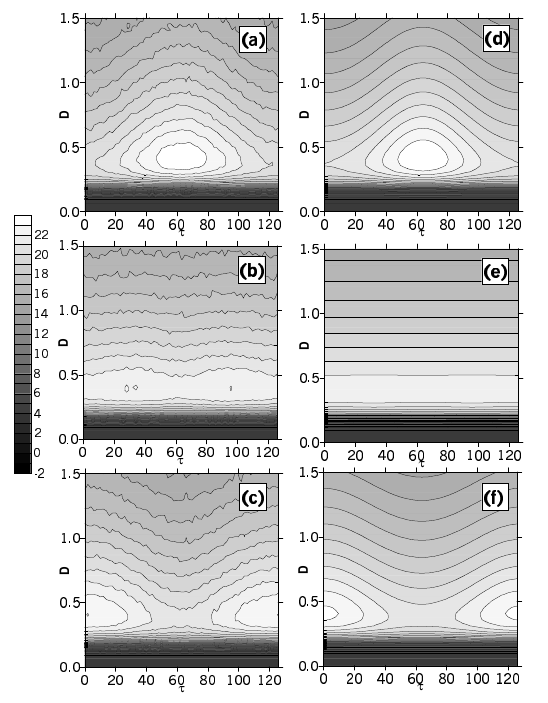
\includegraphics[width=120mm]{images/krawiecki_jezo_1.png}
    \caption{Rys. 1. z pracy \cite{ijmpb_23_2}. Wykresy SNR w zależności od $\tau$ (czas opóźnienia) i D (skalowanie szumu $\eta$. Łańcuch $N=128$ rezonatorów progowych odbierających falę biegnącą, częstotliwość fali $T_s = 128$. Skalowanie wektora falowego $k=\frac{2\pi}{\lambda}$ (a), (d) $\lambda = 2$, (b), (e) $\lambda = 4$, (c), (f) $\lambda = 8$. Lewa kolumna - wyniki symulacji numerycznej, prawa kolumna - wyniki obliczeń teoretycznych}
    \label{fig:graphics:krawiecki_jezo}
  \end{figure}

  \subsubsection{Przestrzennie rozciągły układ neuronów FHN}
  \label{sec:przestrzennie_rozciagly_fhn}

  W modelu FHN, po uwzględnieniu potencjału czynnościowego od połączonych neuronów, równanie na potencjał przedstawia się następująco:

  \begin{equation} \label{eq:v2}
    \epsilon \frac{dv_i}{dt} = v_i(v_i-a)(1-v_i)- \omega + A sin(\beta t) + \eta_i(t) + sv_{ext}(t)
  \end{equation}

  \begin{equation} \label{eq:w2}
    \frac{d \omega_i}{dt} = v_i - d \cdot \omega_i - [b + r sin(\beta t + \phi_i)]
  \end{equation}

  W powyższych równaniach $\phi$ to przesunięcie fazowe pobudzenia periodycznego w danym neuronie, natomiast $v_{ext}$ to łączny potencjał od sąsiadów (pomnożony przez ''czułość'' s):

  \begin{equation}
    v_{ext}(t) = \displaystyle\sum\limits_{n=1}^{k_i} \widetilde{v_{n}}(t-\tau_{n})
  \end{equation}

  Gdzie $\widetilde{v_{n}}(t-\tau_{n})$ to przefiltrowany (patrz niżej) potencjał n-tego sąsiada w chwili $t-\tau_{n}$, a $\tau_{n}$ jest opóźnieniem w transmisji potencjału czynnościowego określonym dla każdej pary neuronów.

  Potencjał przefiltrowany $\widetilde{v_{n}}(t)$, odbierany przez połączone neurony, jest liczony na podstawie ''oryginalnego'' potencjału $v_{n}(t)$ po zaaplikowaniu prostej transformacji progowej zerującej niskie wartości nie kwalifikujące się jako szpilki:

  \begin{equation}
    \tilde{v}(t) = 
    \begin{cases}
      0 & \text{dla } v < \gamma \\
      v(t) & \text{dla } v \geq \gamma 
    \end{cases}
  \end{equation}

  (próg $\gamma = 0.4$)

  Zabieg ten wynika z dynamiki układu FHN, w którym potencjał podprogowy (pomiędzy ''strzałami'') oscyluje wokół wartości wyższej niż zero. Tym samym odbieranie niefiltrowanego, podprogowego potencjału od połączonych neuronów może powodować częste i chaotyczne ''strzały'', niszcząc synchronizację pomiędzy neuronami, co byłoby efektem odwrotnym do zamierzonego.
  
  \subsubsection{Zagadnienia Badane w Pracy}

  Tematem pracy jest badanie zachowania macierzy neuronów FHN. Za pomocą symulacji numerycznej badałem, jak na signal-to-noise ratio wpływa przesunięcie fazowe sygnału periodycznego (rozciągłość przestrzenna układu) oraz parametry wymiany (siła połączenia, opóźnienie transmisji). Ważnym elementem analizy wyników symulacji było porównanie wyników osiągniętych dla modeli neuronów biologicznych (tj. będących przedmiotem niniejszej pracy) z wynikami dla prostych, progowych rezonatorów.

  Badałem układ kilku FHN połączonych w jednowymiarowy sznur. Dla uniknięcia sprzężenia zwrotnego  transmisja sygnału pomiędzy neuronami odbywała się w jedną stronę.
